%!TEX root = nucleare.tex
\section{Parità intrinseca}
Vediamo\marginnote{20-04-1998} cosa si intende per \emph{parità intrinseca} di una particella. Consideriamo una particella libera
che si trova nell'autostato $\ket{\vec{p}}$ dell'operatore quantità di moto. Sappiamo che:

\begin{equation}
 P^2 \ket{\vec{p}} = \ket{\vec{p}} \Rightarrow P\ket{\vec{p}} = \ket{\vec{-p}} \vee P\ket{\vec{p}} = -\ket{\vec{-p}}
\end{equation}

Quindi in generale si può scrivere:
\begin{equation}
 P\ket{\vec{p}} = \eta\ket{\vec{-p}} \quad\text{con} \quad\eta = +1 \quad\text{o} \quad\eta = -1
\end{equation}

Questo vale anche nel caso in cui $\vec{p} = 0$; in questo caso si ha:
\begin{equation}
 P\ket{\vec{p} = 0} = \eta\ket{\vec{p} = 0} \quad (\eta = \pm1)
\end{equation}
Questa è un'equazione agli autovalori, quindi $\eta$ si può interpretare come autovalore della parità intrinseca della
particella. Lo stesso discorso si può fare per l'autostato di una particella senza spin in un campo centrale:
\begin{equation}
 \Psi(\vec{r}) = \chi(\vec{r}) \Psi_e^m(\theta, \varphi)
\end{equation}
In questo caso si ha che:
\begin{equation}
 P\Psi(\vec{r}) = \Psi^{(P)}(\vec{r}) = \eta \Psi(-\vec{r}) \quad (\eta = \pm1)
\end{equation}
Questa è l'espressione più generale. Se si ha $\eta = +1$ la $\Psi(\vec{r})$ si trasforma
come uno scalare; se $\eta = -1$, $\Psi(\vec{r})$ si trasforma come uno pseudoscalare rispetto alla trasformazione di parità.
Dunque si può scrivere:
\begin{equation}
 P\Psi(\vec{r}) = \eta(-1)^l \Psi(\vec{r})
\end{equation}
dove $\eta(-1)^l$ è il complessivo autovalore di parità della particella.

Se una particella è presente sia prima che dopo il processo, la sua parità non può influire sulla conservazione o meno della
parità dell'intero sistema. In questo caso non cambia nulla se si assegna a questa particella un valore $+1$ o $-1$ alla parità.
Si può determinare l'effettiva parità intrinseca di una particella solo se questa viene creata o distrutta nel processo, o più
precisamente quando la sua parità risulta essenziale per la conservazione della parità del sistema nel processo.

Le uniche particelle a cui è possibile assegnare una parità effettiva sono i bosoni, in quanto sono le uniche particelle che
possono essere create o distrutte singolarmente. I fermioni possono essere creati o distrutti sempre in coppia con un altro
antifermione. In questo caso si può misurare solo la loro parità intrinseca relativa (= prodotto della parità).

La teoria di Dirac sul fermione relativistico prevede che per le coppie fermione-antifermione, la parità relativa debba essere
$-1$; questa previsione è confermata dall'esperienza. Per convenzione viene assegnata ai nucleoni e all'elettrone la stessa
parità intrinseca.

Vediamo come si può misurare ad esempio la parità intrinseca del pione negativo. Consideriamo la seguente reazione:
\begin{equation*}
 \pi^- + d \rightarrow n + n
\end{equation*}

Il pione negativo viene catturato dall'atomo di deuterio e si trova in uno stato con momento angolare nullo all'interno
dell'atomo di deuterio. d ha spin 1, quindi il momento angolare totale del sistema $\pi^- + d$ è $1$. Lo stesso è il momento
angolare totale dei due neutroni finali.

Indichiamo con l ed s i valori del momento angolare orbitale e di spin della coppia di neutroni finali. Si possono avere le
seguenti combinazioni:
\begin{equation*}
 (s=0; l=1),\quad (s=1; l=0), \quad (s=1; l=1), \quad (s=1; l=2)
\end{equation*}
Lo stato finale deve però essere antisimmetrico, quindi:
\begin{equation*}
 (-1)^{l+s+1} = -1
\end{equation*}
Questo equivale a scrivere $l+s=$pari.

L'unica possibile combinazione risulta: $s = 1$ e $l = 1$. Quindi all'inizio si ha $l = 0$ e alla fine $l = 1$. La parità orbitale iniziale è $1$, mentre quella finale è $(-1)^1 = -1$.
Quindi la parità orbitale non consente la conservazione della parità nel processo, si deve allora tenere conto della parità
intrinseca.

In base alla conservazione della parità si può scrivere
\begin{gather*}
 \eta_{\pi} \eta_d (-1)^0 = (-1)^1 \quad\quad (\eta_n \eta_n = 1)\quad\Rightarrow \\
\Rightarrow \eta_{\pi} = -\eta_d
\end{gather*}

Dato che il deutone è composto da due neucloni si ha che $\eta_d = 1$, quindi $\eta_{\pi^-} = -1$ è la parità intrinseca del pione
negativo. Anche gli altri due pioni hanno parità $-1$. La funzione d'onda di $\pi^-$ si trasforma come uno pseudoscalare sotto
l'operazione $P$:
\begin{equation*}
\Phi_{\pi}(\vec{r},t) \xrightarrow[P] \quad \Phi_{\pi}^{(P)}(\vec{r},t) = \eta_{\pi} \Phi_{\pi}(-\vec{r},t) =
-\Phi_{\pi}(-\vec{r},t)
\end{equation*}


In modo analogo si assegna una parità intrinseca al fotone considerando come si trasforma la sua funzione d'onda $\vec{A}$ per
effetto dell'inversione spaziale. Si sfrutta l'invarianza dell'Hamiltoniana di interazione elettromagnetica per l'operazione $P$,
cioè rimane invariato il termine $\vec{J}\cdot\vec{A}$; $\vec{J}$ è un vettore polare, cioè
\begin{equation*}
 \vec{J}(\vec{r},t) \xrightarrow[P]{} -\vec{J}(-\vec{r},t)
\end{equation*}
quindi anche per il potenziale vettore deve essere:
\begin{equation*}
 \vec{A}(\vec{r},t) \xrightarrow[P]{} \eta_{\gamma}\vec{A}(-\vec{r},t) = -\vec{A}(-\vec{r},t)
\end{equation*}

Si assegna quindi al fotone una parità intrinseca $\eta_{\gamma} = -1$. Il fotone però non risulta mai a riposo, quindi
l'autovalore di parità del fotone non si riduce mai alla parità intrinseca.

Abbiamo detto che i fermioni si possono creare o distruggere solo in coppia con un antifermione. Una spiegazione di questo si può
trovare nella conservazione del momento angolare totale. Ad esempio se si ha un sistema in cui non ci sono fermioni \footnote{Le
tre parole precedenti si leggono difficilmente. [NdT]} e si crea un fermione, si passerebbe da un valore intero ad uno semintero per il
momento angolare totale.
Sperimentalmente si vede che le coppie sono sempre fermione antifermione. Quindi si ha che in un sistema isolato la differenza
fra il numero di fermioni e di antifermioni è costante nel tempo.

$N_f =$ numero iniziale di fermioni; $N'_f =$ numero finale di fermioni

$N_{\bar{f}} =$ numero iniziale di antifermioni; $N'_{\bar{f}} =$ numero finale di antifermioni.
\begin{equation*}
 N'_f - N'_{\bar{f}} = N_f - N_{\bar{f}}
\end{equation*}

Questa condizione si può scrivere nella forma:
\begin{equation*}
 (+1)N'_f + (-1)N'_{\bar{f}} = (+1)N_f + (-1)N_{\bar{f}}.
\end{equation*}


Si può attribuire ad un fermione o antifermione una carica caratteristica detta \emph{numero fermionico}.

Questa è $+1$ per i fermioni, $-1$ per gli antifermioni o per i bosoni.

La somma algebrica di questa carica in un sistema isolato rimane costante nel tempo:
\begin{equation*}
 (+1)N_f(t) + (-1)N_{\bar{f}}(t) = \text{costante}
\end{equation*}

La legge sperimentale che dice che si possono creare o distruggere solo coppie fermione-antifermione può essere interpretata
come conseguenza della conservazione del numero fermionico.
\chapter{Numeri, quarks e leptoni}
\section{Numero Fermionico Barionico o Numero Barionico}
In un sistema isolato la differenza fra il numero di barioni ($N_b$) e il numero di antibarioni ($N_{b^-}$) è costante nel tempo:
\[
N_b(t)-N_{b^-}(t)=\text{costante}
\]

Questo è un risultato sperimentale. Si può definire un \textit{numero fermionico barionico} ($+1$ per il barione,
$-1$ per l'antibarione, $0$ per le altre particelle) che si conserva:
\begin{equation}
(+1)N_b(t)+(-1)N_b^-(t)=\text{costante}
\end{equation}

Se consideriamo fra i barioni il protone e il neutrone si vede che il numero fermionico barionico si può
identificare con il numero barionico $B$. Infatti $B$ (introdotto nella formula $Q=T_3+\frac{1}{2}B$) è additivo e
si ha che:
\begin{gather}
B|p^+\rangle =(+1)|p^+\rangle\qquad B|n\rangle =(+1)|n\rangle\\
B|p^-\rangle =(-1)|p^-\rangle\qquad B|\bar{n}\rangle =(-1)|\bar{n}\rangle\\
B|\pi\rangle =0
\end{gather}

La legge di conservazione del numero fermionico barionico (o semplicemente numero barionico) assicura la
stabilità del protone (che è il barione più leggero).

Infatti se non si avesse questa legge di conservazione si potrebbero avere i decadimenti:
\[
p^+\rightarrow \pi^0+e^+\qquad p^+\rightarrow \pi^++\nu
\]
Questi sono favorevoli energicamente e conservano tutte le grandezze che si devono conservare, quindi non
avvengono solo per la conservazione del numero barionico.
Questa legge di conservazione è empirica e si applica ad una carica che non ha la stessa valenza fisica della
carica elettrica (che è responsabile di una interazione).
Cioè se questa legge di conservazione non fosse vera non si avrebbero notevoli conseguenze.

\section{Numero quantico di stranezza}
Nel 1947 due fisici, studiando i raggi cosmici, osservarono in una camera a
nebbia le traccie di due processi di decadimento di due nuove particelle.
Queste traccie avevano la configurazione di una V, per questo le particelle si
chiamarono \textit{particelle V}.
Una di queste oggi si chiama \textit{iperone} $\Lambda^0$, decade secondo il
processo:
\[
\Lambda^0\rightarrow p^++\pi^-\qquad\text{è un barione}
\]
mentre l'altra, che si chiama \textit{mesone} $K^0$:
\[
K^0\rightarrow \pi^++\pi^-\qquad\text{è un mesone}
\]

Dalle misure di quantità di moto si stimò la massa di queste particelle:
\[
m_{\Lambda}\simeq 1115,6 \si{\mega\electronvolt}/c^2\qquad m_K\simeq 497,7\si{\mega\electronvolt}/c^2
\]

Si scoprì però che queste particelle avevano un comportamento anomalo.
Queste potevano essere prodotte facilmente con l'urto di un $\pi^-$ e un $p^+$.
D'altra parte avevano un tempo di vita media enormemente più lungo di quello che
ci si poteva aspettare dalle sezioni d'urto di produzione\footnote{Si ha che
tanto è più facile produrre una particella tanto minore sarà il suo tempo di
vita media.}.
Questo sembra contraddire il principio del bilancio dettagliato: se si inverte
il tempo deve essere:
\[
|T_{if}|^2=|T_{fi}|^2\quad (T_{fi}=\text{elemento di matrice della reazione inversa.})
\]

Sperimentalmente le reazioni di produzione sembrano essere:
\begin{gather}
\pi^-+p^+\rightarrow \Lambda^0+?\\
\pi^-+p^+\rightarrow K^0+?
\end{gather}
Cioè nella reazione veniva prodotta una ulteriore particella neutra di cui però
non si conosceva la natura. Si fece prima l'ipotesi che le due reazioni fossero
le seguenti:
\begin{equation}
\pi^-+p^+\rightarrow \Lambda^0+\pi^0\qquad \pi^-+p^+\rightarrow K^0+n
\end{equation}
I dati relativi alla sezione d'urto di produzione di $\Lambda^-$ e $K^-$
fornivano i seguenti valori:
\begin{gather}
\sigma_{\Lambda^0}\simeq\frac{1}{10}\sigma_\text{el}(\pi^--p^+)\\
\sigma_{K^0}\simeq \frac{1}{10}\sigma_\text{el}(\pi^--p^+)
\end{gather}
dove $\sigma_\text{el}(\pi^--p^+)$ è la sezione d'urto del processo di diffusione
elastica forte.
Da questi valori ci si aspettava una vita media di:
\[
\tau_{\text{teor}}=10^{-22}\si{\second}
\]
Sperimentalmente si trovava un tempo di vita media:
\[
\tau_{\text{sper}}=10^{-10}\si{\second}
\]
Questo tempo andava bene per un decadimento di tipo debole, però in base alle
reazioni ipotizzate non vi era motivo di pensare che i processi di decadimento
$\Lambda^0$ e $K^0$
avessero natura diversa dei processi di produzione. Tutto questo portava alla
contraddizione del principio del bilancio dettagliato.
Si ipotizzò, e poi verificò, che $\Lambda^0$ e $K^0$ venivano prodotte solo in
coppia tramite la reazione:
\[
\pi^-+p^+\rightarrow \Lambda^0+K^0
\]

Questa si dice \textit{produzione associata}, e sembrava analoga a quella barione-antibarione.
Questa regola per la produzione portò all'introduzione di una nuova carica:
\textit{numero quantico di stranezza}\footnote{$\Lambda^0$ e $K^0$ devono avere valori
opposti di questo numero quantico.}.
L'interazione forte mostrava quindi di obbedire alla legge di conservazione del
numero quantico di stranezza. Lo stesso però non vale per i processi di
decadimento\footnote{$\pi^-$ e $p^+$ devono avere valore nullo per questo numero
quantico.}.
\[
\Lambda^0\rightarrow p^++\pi^-\qquad K^0\rightarrow \pi^++\pi^-
\]
Quindi questi processi non potevano ritenersi di natura forte. Allora gli
elementi di matrice  del decadimento non avevano niente a che fare con gli
elementi di matrice  del processo di produzione, non si poneva più la questione
del bilancio dettagliato.

Alla luce dei valori sperimentali del tempo di vita media si ipotizzò che i
processi di decadimento fossero di natura debole.
Questo implica che l'interazione debole non verifica la conservazione del numero
quantico di stranezza, e se non vi fosse questa violazione $\Lambda^0$ e $K^0$
risulterebbero stabili.
Supponiamo di assegnare a $\Lambda^0$ stranezza $s=-1$.
Per definire un operatore di stranezza $S=S(Q,T_3,B)$ tale che
\[
S|\Lambda^0\rangle =(-1)|\Lambda^0\rangle
\]
basta considerare che $\Lambda^0$ si presenta in un solo stato di carica
elettrica, e quindi rappresenta un singoletto di isospin. Quindi\footnote{$B=+1$
si deduce dal processo di decadimento.}
\[
Q|\Lambda^0\rangle =0 \quad B|\Lambda^0\rangle =(+1)|\Lambda^0\rangle \quad T_3|\Lambda^0\rangle =0
\]
La relazione $Q=T_3+\frac{B}{2}$ non è valida in questo caso. La relazione esatta è:
\[
Q=T_3+\frac{B+S}{2}
\]
Trovata questa formula si può dedurre il numero quantico di stranezza e quindi anche gli altri numero quantici anche per $K^0$.

\marginnote{24-4-1998} La quantità $B+S$ deve essere uno scalare nello spazio di isospin, in questo modo anche
$S$ sarà uno scalare in questo spazio.
Dalle ipotesi fatte il mesone $K^0$ deve avere un numero quantico di stranezza $S=+1$ (in quanto per $\Lambda^0$ si ha $S=-1$).
Tenendo presente che $B|K^0\rangle =0$ si ha:
\begin{equation}
Q|K^0\rangle =0\quad T_3|K^0\rangle =-\frac{1}{2}|K^0\rangle
\end{equation}
Quindi $K^0$ non può essere uno stato di singoletto di isospin.
Dal momento che $S$ è uno scalare il suo autovalore rimane invariato per una qualsiasi rotazione in questo spazio.
Una qualsiasi rotazione è rappresentata dall'operatore:
\begin{gather}
R_{\tau}=e^{i\theta \hat{u}\cdot\vec{T}}\\
R_{\tau}S=SR_{\tau}\Rightarrow [S,T_-]=0
\end{gather}
dove si era definito $T_+=T_1+iT_2$ e $T_-=T_1-iT_2$.

Se applichiamo $T_+$ allo stato $|K^0\rangle$ si vede che il mesone $K^0$ deve presentarsi con la stessa
stranezza ma con carica diversa.
La carica elettrica di questo nuovo stato sarà $+1$. Il mesone $K^+$ con massa circa uguale a quella del $K^0$
esiste, e viene prodotto dalla reazione forte:
\[
\pi^-+p^+\rightarrow K^++K^-+n
\]
In questa reazione compare il $K^-$, che è l'antiparticella di $K^+$.
Quindi si ha il doppietto di isospin con $S=+1$ ($K^+=+1/2$,$K^0=-1/2$).
Esiste ache l'antidoppietto ($K^-=-1/2$,$K^0=+1/2$) con $S=-1$. Il $\bar{K}^0$ si distingue da $K^0$ in quanto ha
numero quantico di stranezza opposto. La reazione forte che produce il $\bar{K}^0$ è ad esempio:
\begin{equation}
K^-+p^+\rightarrow \bar{K}^0+n
\end{equation}
In definitiva esistono un mesone $K$ e un mesone $\bar{K}$, ciascuno dei quali è rappresentato da un doppietto di isospin.
Sia $K$ che $\bar{K}$ hanno parità intrinseca $-1$, cioè:
\begin{equation}
\eta_{K}=\eta_{\bar{K}}=-1
\end{equation}
Questo è un esempio in cui dalla teoria si può prevedere l'esistenza di una particella (il $K^+$).

Oltre a $\Lambda^0$ e a $K^0$ sono stati trovati altri adroni strani, cioè con stranezza diversa da $0$. In ordine
di massa crescente esistono:
\begin{itemize}
\item Iperone $\sum\equiv (\sum^-,\sum^0,\sum^+)$ $S=-1$. $\sum$ ha spin $1/2\Rightarrow$ è un barione.
\item Iperone $\Xi\equiv (\Xi^-,\Xi^0)$ $S=-2$. $\Xi$ ha spin $1/2\Rightarrow$ è un barione.
\item Iperone $\Omega^-$ $S=-3$.
\end{itemize}

Questi iperoni possono essere prodotti in reazioni del tipo:
\begin{gather}
K^-+p^+\rightarrow \pi^++\sum^-\qquad K^-+p^+\rightarrow K^++\Xi^-\\
K^-+p^+\rightarrow \pi^0+\sum^0\qquad K^-+p^+\rightarrow K^0+\Xi^0\\
K^-+p^+\rightarrow \pi^-+\sum^+\qquad K^-+p^+\rightarrow K^0+\Omega^-
\end{gather}

Tutte queste particelle strane subiscono decadimenti deboli che non conservano la stranezza.
Questi decadimenti verificano la regola di selezione empirica $|\Delta S|=1$. Secondo questa regola non
possono avvenire decadimenti con variazione di stranezza maggiore di $1$.
Ad esempio non possono avvenire i decadimenti:
\begin{equation}
\Xi^0\nrightarrow p^++\pi^-|\;\Xi^-\nrightarrow n+\pi^-|\;\Omega^-\nrightarrow \pi^-+\Lambda^0
\end{equation}
Un'altra regola di selezione verificata dai decadimenti degli adroni strani è:
$\Delta q= \Delta S$ con $\Delta q\neq 0$ dove $\Delta q$ è la variazione di carica
degli adroni. Questa regola non vale nei decadimenti non leptonici, dove cioè non vengono prodotti leptoni, in
quanto si ha $\Delta q=0$. Questa regola vale per decadimenti leptonici (vengono prodotti solo leptoni) e
semileptonici (vengono prodotti leptoni più adroni). Ad esempio non avviene il decadimento:
\begin{equation}
\sum^+ \nrightarrow n+e^+ +\nu\quad \Delta q=-1\quad \Delta S=+1
\end{equation}
mentre è consentito il decadimento:
\begin{equation}
\sum^-\rightarrow n+e^-+\bar{\nu}\qquad \Delta q=\Delta S=+1
\end{equation}

Una spiegazione di queste due regole di selezione è fornito dal modello a quark, cioè gli adroni non sono
particelle semplici, ma composte di quarks.

\section{Numero quantico di incanto}
Un altro numero quantico è il numero quantico di incanto.
Esistono adroni incantati prodotti in processi forti soltanto in coppia,
questi poi decadono con processi deboli senza che si conservi l'incanto.
L'operatore di incanto $I$ è definito dalla formula generalizzata (vedere
\autoref{ch:mesonek}):
\begin{equation}
Q=T_3+\frac{B+S+I}{2}
\end{equation}
Per gli adroni esistono altri due numeri quantici il cui significato fisico, come per la stranezza e l'incanto, è oscuro.

\marginnote{29-4-1998} I processi di decadimento (non leptonici) del mesone $K^+$ sono:
\begin{gather}
K^+\rightarrow \pi^++\pi^0\qquad (R=21\%)\\
K^+\rightarrow \pi^++\pi^++\pi^-\qquad(R=5,6\%)\$\
K^+\rightarrow \pi^++\pi^0+\pi^0\qquad (R=1,7\%)
\end{gather}

Si ha che la vita media del mesone $K^+$ è:
\[
\tau_{K^+}=1,23\cdot 10^{-8}\si{\second}
\]
Il mesone $K^-$ invece non fa in tempo a decadere in quanto viene assorbito da un nucleone circostante secondo la reazione:
\begin{gather}
K^-+N\rightarrow \pi+\Lambda^0\\
K^-+N\rightarrow \pi+\sum
\end{gather}
Il mesone $K^+$, avendo stranezza $+1$, non può invece convertire un nucleone in iperone.
Il $K^+$ subisce in genere processi di scattering elastico da parte dei nuclei.
I processi di decadimento del $K^+$ con due o più pioni non conservano la parità.
Storicamente questa non conservazione non fu compresa subito, infatti si ipotizzò che vi fossero due tipi
di particelle $K^+$ con parità intrinseca opposta.
Questi si indicavano con $\theta^+$ e $\tau^+$. I processi ipotizzati erano:
\[
\theta^+\rightarrow \pi^-+\pi^+\qquad \tau^+\rightarrow 3\pi
\]
Questa interpretazione si rivelò contraddittoria, in quanto i dati sulla produzione forte indicavano un'unica
parità intrinseca. I fisica cinesi Lee e Yang suggerirono una verifica diretta della simmetria per inversione
spaziale per i processi deboli (1956).
Nel 1957 fu fatto l'esperimento della radiazione $\beta$ del Cobalto 60.

Analizziamo ora il decadimento del $K^+$ in due pioni:
\[
K^+\rightarrow \pi^++\pi^0
\]
Supponiamo che il mesone $K^+$ sia a riposo. Tutte le particelle hanno spin zero.
Quindi il numero quantico orbitale dei due pioni finali è $l=0$. Applicando l'operatore parità $P$ si ha:
\begin{equation}
P|\pi^+,\pi^0\rangle=\eta_{\pi}^2(-1)^l|\pi^+,\pi^0\rangle=(+1)|\pi^+,\pi^0\rangle
\end{equation}
Per il decadimento del $K^+$ in tre pioni si ha che il momento angolare totale dei tre pioni si può scrivere come:
\begin{equation}
\vec{J}=\vec{L_{12}}+\vec{L_3}
\end{equation}
dove $\vec{L_{12}}$ è il momento orbitale dei primi due pioni rispetto al loro centro di massa (momento orbitale relativo).
$\vec{L_3}$ è il momento orbitale dell'intero sistema dei primi due pioni\footnote{Come se fossero nel loro C.M.}
più il terzo pione, tutto relativamente al centro di massa dei tre pioni.

Se ipotizziamo sempre che $K^+$ sia inizialmente a riposo allora lo stato finale deve essere un autostato di
$\vec{J}$ con autovalore $j=0$, cioè:
\[
j=j_{\text{min}}=|l_{12}-l_3|=0\Rightarrow l_{12}=l_3
\]
Ricordando che la parità intrinseca di ogni pione è $-1$ si ha che:
\[
P|3\pi\rangle=\eta_{\pi}^3(-1)^{l_{12}}(-1)^{l_3}|3\pi\rangle=(-1)|3\pi\rangle
\]
Quindi uno stesso $K^+$ pur avendo parità intrinseca definita può decadere in stati con parità opposta.
L'interazione responsabile del decadimento\footnote{L'interazione debole.} dunque non conserva la parità.
Il mesone $K^+$ decade anche attraverso canali leptonici e semileptonici, ad esempio:
\begin{gather}
K^+\rightarrow \bar{e}+\nu\quad(\bar{e}=\mu^+,e^+)\quad(R\simeq 63\%)\\
K^+\rightarrow \pi^0+\bar{e}+\nu\qquad(R\simeq 8\%)
\end{gather}
Gli stati finali non hanno una parità definita. Considerando i decadimenti simmetrici si ha:
\begin{gather}
K^+\rightarrow e+\bar{\nu}\quad(e=\mu^-,e^-)\\
K^+\rightarrow \pi^0+e+\bar{\nu}
\end{gather}
A meno di un fattore di fase:
\begin{gather}
|e,\bar{\nu}\rangle =CP|\bar{e},\nu\rangle\\
|\pi^0,e,\bar{\nu}\rangle =CP|\pi^0,\bar{e},\nu\rangle\quad(\mu=\text{muone}=\text{elettrone pesante})
\end{gather}

\section{Gruppo delle matrici unitarie speciali}
Consideriamo un nucleone e indichiamo il suo generico stato di isospin con la funzione d'onda:
\[
\begin{pmatrix}
c_1\\
c_2
\end{pmatrix}
=c_1
\begin{pmatrix}
1\\
0
\end{pmatrix}
+c_2
\begin{pmatrix}
0\\
1
\end{pmatrix}
\]
Dove $c_1$ e $c_2$ sono coefficienti complessi. Questa funzione d'onda si dice
\textit{spinore}. Una generica trasformazione lineare in questo spazio sarà
rappresentata da una matrice complessa.
Sia $U'$ la matrice tale che:
\[
\begin{pmatrix}
c_1'\\
c_2'
\end{pmatrix}
=U'
\begin{pmatrix}
c_1\\
c_2
\end{pmatrix}
\]
Se imponiamo che venga conservata la norma $U'$ deve essere una matrice
unitaria, cioè $U^{'\dagger}U'=I$.
Per il determinante si ha che:
\[
\det(U'^{\dagger}U')=\det(U'^{\dagger})\det(U')=\det(U')^*\det(U')=|\det(U')|^2=1
\]
In generale si può dunque scrivere:
\[
\det(U')=e^{i\theta}\quad\theta\in\mathbb{R}
\]
La matrice unitaria $U'$ si può scomporre nella forma:
\begin{equation}
U'=e^{i\theta/2}U\Rightarrow U=e^{-i\theta/2}U'
\end{equation}
dove $U$ è una matrice unitaria con determinante $+1$. Una matrice con questa
proprietà si dice \textit{matrice unitaria speciale}.
La matrice $U$ è quella che dà luogo al rimescolamento fra i due stati ($p$ e
$n$), in quanto il fattore di fase lascia inalterato il rapporto $c_1/c_2$.

L'insieme della matrici unitarie speciali comprende $I$ e l'inversa di ogni
matrice unitaria speciale. Se $U_1$ e $U_2$ sono unitarie speciali lo è anche
$U_3=U_1U_2$.
Si può concludere che l'insieme delle matrici unitarie speciali costituisce un
gruppo rispetto all'operazione di moltiplicazione fra matrici. Le proprietà di
un gruppo $\mathscr{G}$ sono:
\begin{enumerate}
\item $\forall\,g_1,g_2\in\mathscr{G}\quad g_1g_2=g_3\in\mathscr{G}$
\item $(g_1g_2)g_3=g_1(g_2g_3)=g_1g_2g_3\quad\forall g_1,g_2,g_3\in\mathscr{G}$
\item $\exists !e\in\mathscr{G}:\;\forall g\in\mathscr{G}\quad eg=ge=g$
\item $\forall g\in\mathscr{G}\;\exists !g^{-1}\in\mathscr{G}:\;\;gg^{-1}=g^{-1}g=e$
\end{enumerate}
Il gruppo di matrici unitarie speciali $2\times 2$ si indica col simbolo
$SU(2)$. Questo gruppo è non abeliano, cioè non vale la proprietà commutativa.

\marginnote{4-5-1998} Il gruppo delle matrici unitarie speciali contiene la
matrice idntità. Vediamo come deve essere fatta una matrice infinitamente vicina
a $I_2$ e tale da essere ancora unitaria speciale. Poniamo:
\[
I+i\xi
\]
dove $\xi$ è una matrice $2\times 2$ ad elementi complessi infinitesimi. Quindi
si può scrivere:
\[
I+i\xi=
\begin{pmatrix}
1+i\xi_{11} & i\xi_{12}\\
i\xi_{21} & 1+i\xi_{22}
\end{pmatrix}
\]
Trascuriamo gli infinitesimi del secondo ordine. La condizione di unitarietà è:
\begin{equation}
(I+i\xi)(I-i\xi^{\dagger})=I\Rightarrow I+i\xi-i\xi^{\dagger}=I\Rightarrow \xi=\xi^{\dagger}
\end{equation}
La condizione che il determinante di $I+i\xi$ sia 1 si può scrivere come:
\begin{equation}
det(I+i\xi)=1\Rightarrow (1+i\xi_{11})(1+i\xi_{22})=1\Rightarrow \xi_{11}+\xi_{22}=0
\end{equation}
Quindi la matrice $I+i\xi$ è unitaria speciale se e solo se $\xi$ è hermitiana
con traccia nulla. La matrice $U=I+i\xi$ è univocamente determinata una volta
che sono dati i tre parametri $\epsilon_1,\epsilon_2,\epsilon_3$:
\[
U=U(\epsilon_1,\epsilon_2,\epsilon_3)=I+i\xi(\epsilon_1,\epsilon_2,\epsilon_3)
\]
dove
\[
\begin{split}
&\xi(\epsilon_1,\epsilon_2,\epsilon_3)=\frac{1}{2}
\begin{pmatrix}
\epsilon_3 & \epsilon_1-i\epsilon_2\\
\epsilon_1+i\epsilon_2 & -\epsilon_3
\end{pmatrix}
=\\
&=\frac{1}{2}\epsilon_1
\begin{pmatrix}
0 & 1\\
1 & 0
\end{pmatrix}
+\frac{1}{2}\epsilon_2
\begin{pmatrix}
0 & -i\\
i & 0
\end{pmatrix}
+\frac{1}{2}\epsilon_3
\begin{pmatrix}
1 & 0\\
0 & -1
\end{pmatrix}
=\\
&=\epsilon_1\frac{\tau_1}{2}+\epsilon_2\frac{\tau_2}{2}+\epsilon_3\frac{\tau_3}{2}=\vec{\epsilon}\cdot\vec{T}
\end{split}
\]
Dunque
\begin{equation}
U=U(\epsilon_1,\epsilon_2,\epsilon_3)=I+i\vec{\epsilon}\cdot\vec{T}
\end{equation}
Quindi abbiamo introdotto uno spazio tridimensionale astratto (= spazio di
isospin) dove $\vec{\epsilon}=(\epsilon_1,\epsilon_2,\epsilon_3)$ e $\vec{T}$ è
il vettore di isospin. Riassumendo:
\begin{equation}
U(\epsilon_1,\epsilon_2,\epsilon_3)=I+i\vec{\epsilon}\cdot\vec{T}
\end{equation}
Questa trasformazione unitaria speciale agisce nello spazio di isospin e può
considerarsi associata alla rotazione infinitesima nello spazio tridimensionale
di isospin attorno alla direzione individuata da $\vec{\epsilon}$.
Questa corrispondenza è biunivoca. Se consideriamo una rotazione finita attorno
all'asse $\vec{\epsilon}$ si avranno tre angoli $\theta_1,\theta_2,\theta_3$
tali che:
\[
\epsilon_k=d\theta_k=\lim_{N\to\infty}\frac{\theta_k}{N}\quad(K=1,2,3\;\;N=\text{intero positivo})
\]
A questa rotazione corrisponde la matrice unitaria speciale:
\begin{equation}
U(\theta_1,\theta_2,\theta_3)=\lim_{N\to\infty}(I+i\sum_{k=1}^3\frac{\theta_k}{N}T_k)^N=e^{i\epsilon_k\theta_kT_k}=e^{i\theta\vec{n}\cdot\vec{T}}
\end{equation}
Le matrici $T_1,T_2,T_3$ si possono operativamente scrivere come:
\begin{equation}
T_k=-i\frac{\partial}{\partial\theta_k}U(\theta_1,\theta_2,\theta_3)\bigr\vert_{\theta_1=\theta_2=\theta_3=0}
\end{equation}
$T_k$ si dicono i generatori del gruppo considerato (matrici unitarie speciali).
Si può pure scrivere:
\[
I=U(0,0,0)
\]

Dal momento che una qualsiasi matrice unitaria speciale si può vedere come il
limite del prodotto di matrici unitarie speciali infinitesime, studieremo solo
le proprietà di queste ultime.
Il gruppo delle matrici speciali di ordine 2 viene identificato come un gruppo
di Lie di dimensione 3, cioè:
\begin{equation}
SU(2)=\text{gruppo di Lie di dimensione }3
\end{equation}

Per gruppo di Lie si intende un gruppo continuo i cui elementi $g$ costituiscono
una funzione analitica di un numero finito di parametri indipendenti
$a_1,a_2,\dots,a_n$, che possono variare in modo continuo.
Cioè $g(a_1,a_2,\dots,a_n)$.

Il numero di parametri indipendenti determina la dimensione del gruppo di Lie.
Nel caso di $SU(2)$ è evidente perchè la dimensione è
3\footnote{$g(\epsilon_1,\epsilon_2,\epsilon_3)$}.
Tutti gli elementi di un gruppo di Lie di dimensione n possono ricavarsi dagli
elementi $g(\epsilon_1,\epsilon_2,\dots,\epsilon_n)$ che sono infinitamente
vicini a $g(0,0,\dots,0)$ che è l'elemento identità.
Basterà dunque conoscere i generatori del gruppo:
\begin{equation}
I_k=\frac{\partial}{\partial a_k}g(a_1,a_2,\dots ,a_n)\bigr\vert_{a_1=a_2=\dots =a_n=0}\qquad (k=1, 2, \dots , n)
\end{equation}
Le proprietà del gruppo di Lie dipendono dalle proprietà dei generatori. Nel
caso del gruppo $SU(2)$ i tre generatori $T_1,T_2,T_3$ obbediscono alle regole
di commutazione $[T_i,T_j]=i\epsilon_{ijk}T_k$ ($i,j,k=1,2,3$).

Queste regole costituiscono l'algebra del gruppo di Lie nel gruppo $SU(2)$.
I numeri $\epsilon_{ijk}$ si dicono \textit{costanti di struttura del gruppo}.
Esiste una corrispondenza biunivoca fra le matrici delle rotazioni dello spazio
di isospin e le matrici $U(\theta_1,\theta_2,\theta_3)$, e anche le matrici
delle rotazioni sono un gruppo di Lie.

Sia dato un gruppo $\mathscr{G}$ con elementi $g$ e sia dato uno spazio
vettoriale lineare $L$ dove è definito l'insieme degli operatori $T(g)$.
Questo insieme di operatori è una rappresentazione del gruppo $\mathscr{G}$
nello spazio lineare $L$ se vale la relazione:
\[
T(gg')=T(g)T(g')\qquad \forall g,g'\in\mathscr{G}
\]
La dimensione di $L$ determina la dimensione di tale rappresentazione.
Nel nostro caso abbiamo che:
\begin{gather}
g=g(\theta_1,\theta_2,\theta_3)=\text{matrice della rotazione nello spazio di isospin}\\
T(g)=U(\theta_1,\theta_2,\theta_3)=\text{rotazione nello spazio degli stati di isospin $1/2$}\\
L=\text{spazio degli stati di isospin $1/2$}
\end{gather}
Un gruppo può avere più di una rappresentazione.
Il gruppo delle rotazioni dello spazio di isospin ha un numero infinito di
rappresentazioni di dimensione $2t+1$.

La rappresentazione che permette di costruire tutte le altre rappresentazioni si
dice \textit{rappresentazione fondamentale}, e la base su cui tale
rappresentazione agisce si dice \textit{multipletto fondamentale}.

Nel nostro caso la rappresentazione fondamentale delle rotazioni è costituita
dalle matrici speciali $2\times 2$.
I due stati $|p\rangle$ e $|n\rangle$ sono il multipletto fondamentale.
Le matrici unitarie speciali $SU(2)$ costituiscono anche una rappresentazione di
se stesse.
Le matrici unitarie speciali $2\times 2$ sono la rappresentazione fondamentale
di se stesse.

\marginnote{6-5-1998} Per qualunque rappresentazione di un gruppo di Lie si ha
la stessa algebra.
Consideriamo i tre generatori della rappresentazione fondamentale
$T_k=(T_k)^{1/2}$ con $k=1,2,3$ del gruppo $SU(2)$. Indichiamo con
\[
\psi^{1/2}=
\begin{pmatrix}
\psi_p\\
\psi_n
\end{pmatrix}
\]
la funzione d'onda di isospin. Una rotazione dello spazio di isospin individua una trasformazione nello spazio degli stati:
\begin{equation}
\psi'^{1/2}=e^{i\theta\vec{n}\cdot\vec{T}}\psi^{1/2}
\end{equation}
Questa si può generalizzare nel caso in cui si ha un generico $t$. La dimensione dello spazio degli stati è $2t+1$ e si ha:
\[
\psi'(t)=e^{i\theta\vec{n}\cdot\vec{T}(t)}\psi(t)
\]
Mentre il numero di generatori è sempre tre, questi generatori sono $T_1^{(t)},T_2^{(t)},T_3^{(t)}$ che
sono relativi alla rappresentazione considerata, infatti sono matrici di ordine $2t+1$.
Questi generatori seguono la stessa algebra di quelli nel caso $t=1/2$, quindi si può scrivere:
\begin{equation}
[T_i^{(t)},T_j^{(t)}]=i\epsilon_{ijk}T_k^{(t)}
\end{equation}
Il multipletto fondamentale di isospin è $(|p\rangle,|n\rangle)$. Questo si può
riscrivere in modo compatto con il simbolo $\Ci{2} \equiv (|p\rangle,|n\rangle)$.

Sappiamo che il prodotto diretto di due distinti doppietti di isospin dà una basa di quattro stati, un tripletto e
un singoletto, e si scrive:
\[
\Ci{2}\times\Ci{2}=\Ci{3}+\Ci{1}
\]
Consideriamo lo spazio definito dalla base $\Ci{2}_a\times\Ci{2}_b$ e analizziamo la rappresentazione di ordine
4. La matrice identità è:
\[
I=I_a\times I_b\quad(\text{$I_a$ e $I_b$ trasformazioni identità nelle basi $\Ci{2}_a$ e $\Ci{2}_b$})
\]
Consideriamo una matrice unitaria speciale infinitamente vicina a $I$:
\begin{equation}
\begin{split}
&U(\epsilon_1,\epsilon_2,\epsilon_3)=(I_a+i\vec{\epsilon}\cdot\vec{T})(I_b+i\vec{\epsilon}\cdot\vec{T_b})=\\
&I+i\vec{\epsilon}\cdot(\vec{T}_a\times I_b+I_a\times\vec{T}_b)
\end{split}
\end{equation}
I generatori di questa rappresentazione sono $\vec{T}=\vec{T}_a\times I_b+I_a\times\vec{T}_b$.

La generica trasformazione che appartiene alla rappresentazione si può scrivere nella forma:
\[
e^{i\theta\vec{n}\cdot\vec{T}}=e^{i\theta\vec{n}\cdot(\vec{T}_a\times I_b+I_a\times\vec{T}_b)}
\]
Vale anche la proprietà:
\[
[\vec{T}^2,e^{i\theta\vec{n}\cdot\vec{T}}]=0
\]
Questo garantisce che gli elementi della trasformazione lasciano invariato il numero quantico $t$, quindi non si
può avere un passaggio dal sottospazio di singoletto a quello di tripletto (e viceversa) tramite queste
trasformazioni.
Lo spazio su cui agisce la rappresentazione è quindi scomponibile in due sottospazi invarianti, $t=1$ e $t=0$.
Si tratta dunque di una rappresentazione riducibile, cioè scomponibile in due rappresentazioni, una agente nello
spazio di tripletto e l'altra in quello di singoletto.
Se scegliamo come base quella costituita dai componenti del tripletto e del singoletto la rappresentazione
assumerà la forma diagonale a blocchi:
\[
e^{i\theta\vec{n}\cdot\vec{T}}=
\begin{pmatrix}
e^{i\theta\vec{n}\cdot\vec{T}^{(1)}} & 0\\
0 & e^{i\theta\vec{n}\cdot\vec{T}^{(0)}}
\end{pmatrix}
=
\begin{pmatrix}
e^{i\theta\vec{n}\cdot\vec{T}^{(1)}} & 0\\
0 & 1
\end{pmatrix}
\]
Una rappresentazione che agisce in uno spazio vettoriale $L$ si dice riducibile se esiste almeno un sottospazio di
$L$ in cui rimane invariante, in caso contrario si dice irriducibile.

Tutto quanto detto si può generalizzare nel caso di un gruppo $SU(n)$.
La dimensione di queste matrici è $n$. Una matrice unitaria speciale infinitamente vicina a $I$ si può scrivere come
\[
U=I+i\xi
\]
dove $\xi$ è una matrice $n\times n$ a elementi complessi, hermitiana e a traccia nulla. Questa sarà individuata da
$n-1$ elementi indipendenti reali sulla diagonale, e da $\frac{n^2-n}{2}$ elementi indipendenti complessi non
diagonali.
Quindi il numero totale di parametri indipendenti è:
\[
(n-1)+2(\frac{n^2-n}{2})=n-1+n^2-n=n^2-1
\]
Indichiamo questi $N^2-1$ elementi con $\epsilon_1,\epsilon_2,\dots,\epsilon_{n^2-1}$.
La matrice $\xi$ si può dunque scrivere nella forma:
\begin{equation}
\xi=\sum_{k=1}^{n^2-1}\epsilon_kT_k
\end{equation}
dove i $T_k$ sono gli $n^2-1$ generatori.
La trasformazione generica appartenente alla rappresentazione di $SU(n)$ è:
\begin{equation}
U(\theta_1,\theta_2,\dots,\theta_{n^2-1})=\exp[i\sum_{k=1}^{n^2-1}\theta_kT_k]
\end{equation}
Il gruppo $SU(n)$ è un gruppo di Lie di dimensione $n^2-1$, la cui rappresentazione fondamentale ha
dimensione $n$.
Il numero di generatori del gruppo e di tutte le sue rappresentazioni è $n^2-1$.

\section{Teoria dei Quarks}
\marginnote{8-5-1998} Uno dei principali obiettivi della fisica di oggi è quello
di trovare un ordinamento fra le particelle.
Una scuola di pensiero considera le particelle tutte con la stessa elementarità,
mentre una seconda che si ispira alla tavola periodica degli elementi non le
considera tutte egualmente elementari.

Nel 1956 Sakata ipotizzò che tutti gli adroni conosciuti fossero combinazioni di
tre particelle: $n,p^+,\Lambda^0$ (e le corrispondenti antiparticelle).
\begin{gather}
n=\text{portatore di numero barionico.}\\
p^+=\text{portatore di carica elettrica elementare.}\\
\Lambda^0=\text{portatore del numero quantico di stranezza}.
\end{gather}

Presto si vide che questo modello era in disaccordo con l'esperienza in quanto
prevedeva l'esistenza di particelle mai evidenziate sperimentalmente.
Ad esempio consideriamo l'esistenza di iperoni con stranezza
positiva:$p^+n\bar{\Lambda}^0$, questi in realtà non esistono.

Subito dopo fu messo in luce che tutti gli adroni conosciuti potevano essere
raggruppati secondo lo spin e la parità intrinseca in famiglie da $1,8,10$
componenti.
\[
Y=B+S\quad\text{ipercarica}\quad\text{S = stranezza, B = num. barionico}
\]
Per i barioni con spin $1/2$ e i mesoni di spin $0$ rientrano tutti in un
ottetto (schemi in \autoref{fig:ott}).
\begin{figure}[!h]
  \caption{Ottetti.}
  \label{fig:ott}
  \subfloat[][Ottetto barionico (barioni con spin
  1/2)]{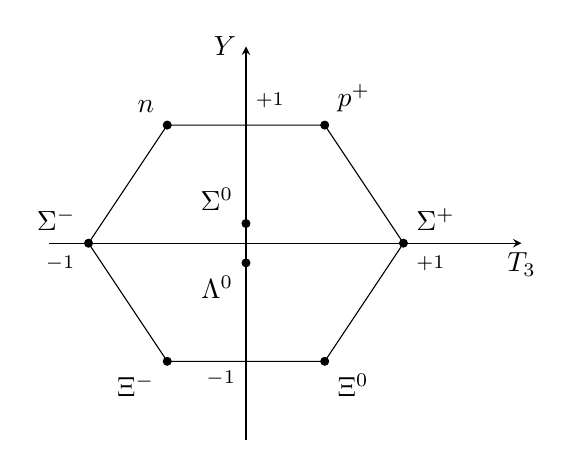
\begin{tikzpicture}[>=stealth,
  punto/.style={circle, draw=\MinorColor, fill=\MinorColor, inner sep=1pt}]
  \draw[->] (-2.5,0) -- (3.5,0) node [below] {$T_3$};
  \draw[->] (0,-2.5) -- (0,2.5) node [left] {$Y$};
  \draw (1,1.5) node [punto, label=above right:$p^+$] {}
     -- (2,0) node [punto, label=below right:$^{+1}$, label=above right:$\Sigma^+$] {}
     -- (1,-1.5) node [punto, label=below right:$\Xi^0$] {}
     -- (-1,-1.5) node [punto, label=below left:$\Xi^-$] {}
     -- (-2,0) node [punto, label=below left:$^{-1}$, label=above left:$\Sigma^-$] {}
     -- (-1,1.5) node [punto, label=above left:$n$] {} -- cycle;
  \node (a) at (0,1.5) [above right] {$^{+1}$};
  \node (b) at (0,-1.5) [below left] {$^{-1}$};
  \node (s) at (0,.25) [punto, label=above left:$\Sigma^0$] {};
  \node (l) at (0,-.25) [punto, label=below left:$\Lambda^0$] {};
\end{tikzpicture}
}
  \subfloat[][Ottetto mesonico (mesoni con spin $0$)]{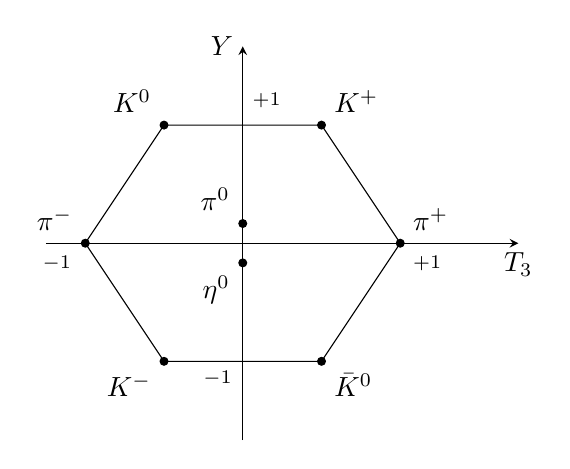
\begin{tikzpicture}[>=stealth,
  punto/.style={circle, draw=\MinorColor, fill=\MinorColor, inner sep=1pt}]
  \draw[->] (-2.5,0) -- (3.5,0) node [below] {$T_3$};
  \draw[->] (0,-2.5) -- (0,2.5) node [left] {$Y$};
  \draw (1,1.5) node [punto, label=above right:$K^+$] {}
     -- (2,0) node [punto, label=below right:$^{+1}$, label=above right:$\pi^+$] {}
	 -- (1,-1.5) node [punto, label=below right:$\bar{K}^0$] {}
     -- (-1,-1.5) node [punto, label=below left:$K^-$] {}
     -- (-2,0) node [punto, label=below left:$^{-1}$, label=above left:$\pi^-$] {}
     -- (-1,1.5) node [punto, label=above left:$K^0$] {} -- cycle;
  \node (a) at (0,1.5) [above right] {$^{+1}$};
  \node (b) at (0,-1.5) [below left] {$^{-1}$};
  \node (p) at (0,.25) [punto, label=above left:$\pi^0$] {};
  \node (e) at (0,-.25) [punto, label=below left:$\eta^0$] {};
\end{tikzpicture}
}
\end{figure}

$\eta^0$ è un mesone di massa $m\simeq549\si{\mega\electronvolt}/c^2$, viene
prodotto nella reazione:
\[
K^-+p^+\rightarrow \eta^0+\Lambda^0
\]
Effettivamente gli adroni potevano quindi raggrupparsi in multipletti composti
da $1,8,10$ componenti. Quelli di sopra sono due esempi.
Questa classificazione è più generale di quella dello spin isotopico. Questa
classificazione si dice \textit{ottuplice via}.
Questa presupponeva per l'interazione forte una simmetria più ampia di quella di
isospin. Nell'ambito di questa simmetria lo spazio a 2 dimensioni degli stati di
isospin deve essere sostituito con uno spazio a 3 dimensioni, in quanto si deve
considerare l'ulteriore grado di libertà associato alla stranezza $-1$.

I tre autostati di isospin e stranezza, pur avendo le stesse prerogative degli stati
$|p^+\rangle,|n\rangle,|\Lambda^0\rangle$, non potevano coincidere con questi in
quanto questi ultimi appartenevano
ad un ottetto.
Si passa così dal gruppo $SU(2)$ caratterizzato da 3 generatori e da un
multipletto fondamentale a 2 dimensioni, al
gruppo $SU(3)$ con 8 generatori ed un multipletto fondamentale a 3 dimensioni
(indichiamo questo con $\Ci{3}$). Si può scrivere:
\begin{equation}
\Ci{3}\times\Ci{3}\times\Ci{3}=\Ci{10}+\Ci{8}+\Ci{8}+\Ci{1}
\end{equation}
A destra sono indicati i supermultipletti in cui l'insieme delle combinazioni
viene a scindersi.

I supermultipletti generano sottospazi invarianti per trasformazioni del gruppo
$SU(3)$. Indicando con $\Ci{$\bar{3}$}$ l'antimultipletto, i multipletti mesonici
si possono ricavare dalle combinazioni:
\[
\Ci{3}\times\Ci{$\bar{3}$}=\Ci{8}+\Ci{1}
\]
Non sembravano esserci particelle corrispondenti ai tre stati dei multipletti,
quindi si pensava che fossero delle strutture fittizie e matematiche degli stati
che non erano occupati da alcuna particella.
Secondo quest'idea gli adroni non erano composti da altre particelle più
elementari e quindi la fisica degli adroni non doveva essere il risultato di una
fisica più elementare.

I due fisici Gell-Mann e Zweig nel '64 avanzarono l'ipotesi che agli stati costituenti il multipletto fondamentale
di $SU(3)$ corrispondessero effettivamente tre entità fisiche con determinati numeri quantici.
Solo con questa ulteriore ipotesi secondo loro si spiegava in maniera completa la fisica degli adroni. Questi
costituenti furono chiamati \textit{quark}:
\begin{equation}
\begin{split}
&\text{quark}\;u (\text{up})\;\;\text{I primi due formano un doppietto di isospin con stranezza $0$.}\\
&\text{quark}\;d (\text{down})\\
&\text{quark}\;s (\text{strange})\;\;\text{singoletto di isospin con stranezza $-1$.}
\end{split}
\end{equation}
Quindi si deve avere:
\begin{gather}
T_3|u\rangle=+\frac{1}{2}|u\rangle\\
T_3|d\rangle=-\frac{1}{2}|d\rangle\\
S|u\rangle=S|d\rangle=0\\
\vec{T}|s\rangle=T_3|s\rangle=0\\
S|s\rangle=-1|s\rangle
\end{gather}

Attribuendo ai quark spin $1/2$ si ricava subito che i barioni di spin $1/2$ dovevano essere costituiti da
combinazioni di 3 quarks di cui due in uno stato di spin di singoletto.
Si deve escludere che uno dei tre quarks possa essere un antiquark, in quanto non verrebbero riprodotti
gli ottupletti esistenti e in più dovrebbero esistere barioni con stranezza positiva.
Ponendo i tre quarks sullo stesso piano si deve attribuire loro un numero barionico pari a $1/3$:
\begin{equation}
B|u\rangle=+\frac{1}{3}|u\rangle\quad B|d\rangle=+\frac{1}{3}|d\rangle\quad
B|s\rangle=+\frac{1}{3}|s\rangle
\end{equation}
Conseguenza di questo è l'attribuzione di una carica elettrica frazionaria, e cioè $+2/3$ per il quark $u$, e
$-1/3$ per i quarks $d$ e $s$.
\begin{equation}
Q|u\rangle=+\frac{2}{3}|u\rangle\quad Q|d\rangle=-\frac{1}{3}|d\rangle\quad Q|s\rangle=-\frac{1}{3}|s\rangle
\end{equation}
Questo si evince dalla formula $Q=T_3+\frac{1}{2}(B+S)$.

Secondo questo modello i barioni sarebbero la combinazione di tre quarks:
\[
\Ci{3}\times\Ci{3}\times\Ci{3}=\Ci{10}+\Ci{8}+\Ci{8}+\Ci{1}
\]
e questa ora non è più un'uguaglianza solo matematica, ma anche fisica.

\marginnote{11-5-1998} Riassumendo quanto detto per barioni e mesoni si ha:
\begin{gather}
\text{barioni}\quad \Ci{3}\times\Ci{3}\times\Ci{3}=\Ci{10}+\Ci{8}+\Ci{8}+\Ci{1}\\
\text{mesoni} \quad \Ci{3}\times\Ci{$\bar{3}$}=\Ci{8}+\Ci{1}\\
\Ci{3}\equiv(|u\rangle,|d\rangle,|s\rangle)\quad \Ci{$\bar{3}$}\equiv(|\bar{u}\rangle,|\bar{d}\rangle,|\bar{s}\rangle)
\end{gather}
Vediamo ora quali sono le combinazioni di quarks che formano $p^+,n,\Lambda^0$:
\begin{equation}
p^+\equiv uud\quad n\equiv ddu\quad \Lambda^0\equiv uds
\end{equation}
Per i mesoni invece si ha:
\begin{equation}
\begin{split}
&\pi^-\equiv d\bar{u}\quad \pi^0\equiv\frac{1}{\sqrt{2}}(u\bar{u}-d\bar{d})\quad \pi^+\equiv u\bar{d}\quad\;\,(s=-1)\\
&K^0\equiv d\bar{s}\quad K^+\equiv u\bar{s}\quad \bar{K}^0\equiv s\bar{d}\quad K^-\equiv s\bar{u}
\end{split}
\end{equation}

La combinazione quark-antiquark per i mesoni è in accordo col fatto che tutti i mesoni con spin $0$ hanno parità
intrinseca negativa.

Questo è il modello a quark proposto nel 1964 da Gell-Mann e Zweig, questo si basa sul gruppo di simmetria
$SU(3)$. Un modello a quark più aggiornato è quello che considera anche un quarto quark, il quark $c$
(``charm''=incanto),
che ha sempre numero barionico $1/3$, numero quantico di incanto $+1$, carica elettrica $+2/3$, isospin $0$ e stranezza $0$.
Cioè questo quark ha la prerogativa di portare il numero quantico di incanto. In questo modo il tripletto
fondamentale va sostituito con un quadrupletto fondamentale ($u,d,s,c$).

Si passa così dalla simmetria $SU(3)$ a $SU(4)$. I barioni derivano da combinazioni
$\Ci{4}\times\Ci{4}\times\Ci{4}$, mentre i mesoni da $\Ci{4}\times\Ci{$\bar{4}$}$.
Oggi si sa che esistono altri due quarks: $t$ (``truth''=verità) e $b$ (``beauty''=bellezza).
Quindi il gruppo di simmetria dell'interazione forte è $SU(6)$.

In realtà non si è mai osservato un quark in modo diretto. L'ipotesi dei quarks è però indirettamente convalidata
da numerosi fatti sperimentali che non si potrebbero spiegare altrimenti.
Uno di questi fatti è la mancanza di barioni con stranezza positiva: questo si spiega con l'esistenza solo di un
quark con stranezza $-1$.
Un altro fatto è la non esistenza di multipletti adronici con numero quantico di isospin maggiore di $3/2$.
I quarks $u$ e $d$ hanno isospin $1/2$, mentre tutti gli altri hanno zero, quindi combinando tre quarks, al più si
può ottenere un $t=3/2$.

Un ulteriore esempio è l'assenza di barioni con stranezza $-1$ e carica $+2$, questo è dovuto al fatto che $s$ ha
carica $-1/3$ e i quarks con carica positiva hanno carica $+2/3$.
Dunque combinando un quark $s$ con altri due quarks la carica maggiore che si può ottenere è $+2/3+2/3-1/3=1$.
L'esistenza del quark $s$ consente di spiegare le due regole empiriche:
\[
|\Delta S|=1\qquad \Delta S=\Delta q\qquad (\Delta q\neq 0) 
\]
che seguono i decadimenti deboli.
Nel modello di G-Z qualsiasi processo di decadimento con variazione di stranezza deve corrispondere ad una
della quattro transizioni:
\begin{gather}
s\rightarrow u\;\;(\Delta S=1,\Delta q=1)\\
s\rightarrow \bar{u}\;\;(\Delta S=-1,\Delta q=-1)\\
s\rightarrow d\;\;(\Delta S=1,\Delta q=0)\\
s\rightarrow \bar{d}\;\;(\Delta S=-1,\Delta q=0)
\end{gather}

Si deve sottolineare però che il modello a quarks prevede sezioni d'urto dei processi di scattering leptone-adrone
in perfetto accordo coi dati sperimentali.
Per verificare questo si usano come particelle incidenti elettroni e neutrini con energia maggiore
di $1\si{\giga\electronvolt}$, che corrisponde ad una lunghezza d'onda di De Broglie \textcrlambda$\,\gtrsim
10^{-14}\si{\centi\meter}$.
Questi sono prevalentemente processi anelastici, i dati sperimentali mostrano che elettroni e neutrini
vengono diffusi da oggetti puntiformi all'interno degli adroni.

Questi dati sono spiegati abbastanza bene dal \textit{modello a partoni} di Feynman. Secondo questo modello
ogni adrone è composto apparentemente da un numero infinito di particelle puntiformi con spin $1/2$ (i
\textit{partoni}).
Queste particelle comprendono i tre quarks reali e una nube d infinite coppie virtuali quark-antiquark, che vestono
i quarks reali (questi si dicono quarks vestiti).

L'indiretta conferma sperimentale dei quarks pone in primo piano la questione della loro inosservabilità; questo si
può spiegare con il confinamento dei quarks all'interno degli adroni dovuto ad un potenziale che cresce molto
rapidamente all'aumentare della distanza fra i quarks (come un potenziale di tipo elastico).
Si può pensare che i quarks siano legati fra loro da molle perfette, in modo che la forza fra i quarks è nulla
per distanze molto piccole, questo consente ai quarks confinati negli adroni di comportarsi come particelle quasi
libere ciascuna con la sua individualità.
Questa proprietà si dice \textit{libertà asintotica}. Questo porta all'assegnazione di una massa ai quarks:
\begin{gather}
m_u=m_d=336\,\si{\mega\electronvolt}/c^2\\
m_s=538\,\si{\mega\electronvolt}/c^2\\
m_c=1650\,\si{\mega\electronvolt}/c^2
\end{gather}

La considerevole differenza di massa fra i quarks rispecchia quella esistente fra gli adroni di uno stesso supermultipletto;
questa differenza è 100 volte superiore a quella attribuibile all'interazione elettromagnetica.
Se denominiamo con interazione forte quella che rispetta la simmetria all'interno di un multipletto allora
esisterà un'altra interazione intermedia fra forte ed elettromagnetica responsabile della differenza di massa fra
le particelle di un supermultipletto.
Questa si dice \textit{interazione medio-forte}; questa continua a rispettare la simmetria di isospin in quanto le
differenze di massa in un multipletto sono dell'ordine di grandezza elettromagnetico.

\section{Numero quantico di colore}
Si notò presto che l'ipotesi dei quarks in alcuni casi contraddiceva il principio di esclusione di Pauli.
Infatti alcuni barioni risultavano costituiti da tre quarks identici nello stesso stato quantico. Ad esempio
consideriamo l'iperone $\Omega^-$ che ha stranezza $-3$ e appartiene al decupletto barionico di spin $3/2$.
L'esistenza di $\Omega^-$ come membro di tale decupletto era stata già prevista dal modello dell'ottuplice via (per
tale previsione Gell-Mann prese il Nobel).
Nel modello a quarks $\Omega^-$ dovrebbe risultare dalla composizione di tre quarks $s$ con spin paralleli e
momento angolare orbitale nullo.
Un altro modello era quello della risonanza barionica $\Delta^{++}$ con spin $3/2$, stranezza $0$ e terza
componente di isospin $3/2$.
Questa risonanza sembrava dover provenire dalla combinazione di tre quarks $u$ con spin paralleli e momento
angolare orbitale nullo.

Chiamiamo \textit{sapore} (flavuor) il numero quantico elementare che distingue un quark da un altro all'interno
del multipletto fondamentale.
Con questo numero quantico si intende in generale un numero quantico di isospin, di stranezza o di incanto.

Cioè ogni quark nel multipletto fondamentale ha un certo sapore. Si pò assumere che la funzione d'onda complessiva
di uno stato di tre quarks sia data dal prodotto di tre fattori:
\begin{equation}
\psi=\psi_l\psi_s\psi_f
\end{equation}
dove
\begin{itemize}
\item $\psi_l$ è la parte spaziale;
\item $\psi_s$ è la parte dipendente dalle coordinate di spin dei quarks;
\item $\psi_f$ è la parte dipendente dalle coordinate di sapore dei quarks.
\end{itemize}

Per l'iperone $\Omega^-$ e $\Delta^{++}$ tutti e tre i fattori risulterebbero simmetrici per lo scambio di due
quarks, così anche $\psi$ risulta simmetrica, invece che antisimmetrica come richiesto dalla statistica di
Fermi-Dirac.
Quindi $\Omega^-$ e $\Delta^{++}$ violano la statistica di F-D. Per ovviare a questa contraddizione nel
'64 Grundberg introdusse un nuovo numero quantico additivo, il \textit{colore}.
Secondo il suo modello i tre quarks che formano $\Omega^-$ e $\Delta^{++}$ sarebbero caratterizzati da diversi
numeri quantici di colore. Cioè pur avendo lo stesso sapore questi avrebbero diverso colore,
e quindi i loro stati quantici non risulterebbero identici.
La funzione d'onda totale di un sistema di tre quarks assume la forma generalizzata:
\begin{equation}
\psi=\psi_l\psi_s\psi_f\psi_c
\end{equation}
dove $\psi_c$ è un fattore che dipende dalle coordinate di colore dei quarks.

Se tre quarks differiscono solo per il colore non risulta più violato il principio di Pauli.
Si può pensare ai tre quarks come a tre particelle non proprio identiche, ma distinguibili per il colore.
Alternativamente si possono immaginare i tre quarks come particelle identiche, cioè che il numero quantico di
colore si può pure scambiare, in questo caso deve valere la statistica di Fermi-Dirac e quindi il fattore $\psi_c$
deve risultare antisimmetrico per lo scambio di due colori.

Qualunque barione nel suo complesso però non appare colorato, cioè non è possibile attribuirgli un numero
quantico diverso da zero, in quanto questo numero quantico non ha alcuna manifestazione fino ad ora. Quindi
assumiamo che ogni barione abbia colore zero e che quindi si trovi in uno stato di singoletto.
Per non contraddire il principio di Pauli ciascun quark deve poter esistere in tre varietà di colore (di solito si
chiamano rosso, verde e blu).
Le funzioni d'onda di questi autostati si indicano con $q_r,q_v,q_b$.
\begin{equation}
\psi_c=\frac{1}{\sqrt{3}}\sum_P(-1)^{n_P}q_r(P_1)q_v(P_2)q_b(P_3)
\end{equation}
Dove P=permutazioni dell'insieme $(1,2,3)\rightarrow(P_1,P_2,P_3)$; $n_P=\,$ parità della permutazione.

Questa $\psi_c$ rappresenta il fattore di colore per tutti i barioni, cioè è lo stato di singoletto con colore
zero, cioè si suppone che rosso+verde+blu= zero.
ogni quark ha la stessa probabilità di avere colore r, v o b, ma il barione è sempre neutro per il colore.

Estendendo l'ipotesi di singoletto di colore anche per i mesoni si trova che la funzione d'onda di colore è:
\begin{equation}
\psi_c=\frac{1}{\sqrt{3}}(q_r\bar{q}_{\bar{r}}+q_v\bar{q}_{\bar{v}}+q_b\bar{q}_{\bar{b}})
\end{equation}
dove $\bar{r},\bar{v},\bar{b}$ sono gli anticolori, che annullano i colori: $r+\bar{r}=0$.

L'ipotesi del colore triplica il numero di quarks in quanto ogni quark con un dato sapore può esistere con tre diversi colori.
L'idea del colore però non implica una variazione di massa in corrispondenza di una variazione di colore.
Appare quindi naturale introdurre una nuova simmetria interna, che è esatta; questa simmetria è caratterizzata
da trasformazioni unitarie con $det=+1$ nello spazio elementare degli stati di colore, spazio definito dal
multipletto fondamentale $|r\rangle,|v\rangle,|b\rangle$.

Questa simmetria esprime l'indipendenza di tutte le interazioni dal colore.

\marginnote{15-5-1998} Se indichiamo con $R_c$ una qualsiasi trasformazione unitaria con $det=+1$ agente nello
spazio degli stati di colore, l'hamiltoniana del sistema non cambia per effetto di questa trasformazione, cioè:
\[
[R_c,H_{\text{TOT}}]=0
\]
Questo equivale ad affermare l'indipendenza di tutte le interazioni rispetto al colore.

Formalmente questa simmetria è analoga a quella di G-Z rispetto alle trasformazioni $SU(3)_f$ agenti nello
spazio individuato dal multipletto di sapore ($|u\rangle,|d\rangle,|s\rangle$).
Quindi si può considerare il multipletto ($|r\rangle,|v\rangle,|b\rangle$) e la simmetria $SU(3)_c$. La
simmetria $SU(3)_f$ non è però esatta, in quanto è rispettata solo dall'interazione forte. Se $R_f$ è una
trasformazione di $SU(3)_f$ si ha:
\begin{equation}
[R_f,H_{\text{TOT}}]\neq 0\qquad[R_f,H_{\text{FORTE}}]=0
\end{equation}
L'identità formale fra simmetria di colore e di sapore suggerirebbe l'esistenza di diversi supermultipletti
di colore in analogia con quelli di sapore. Sia $\Ci{3}_c$ la base di colore:
$\Ci{3}_c=(|r\rangle,|v\rangle,|b\rangle)$. Risulta quindi:
\begin{equation}
\Ci{3}_c\times\Ci{3}_c\times\Ci{3}_c=\Ci{10}_c+\Ci{8}_c+\Ci{8}_c+\Ci{1}_c
\end{equation}
Si ritiene tuttavia che la totalità degli adroni osservabili deve occupare il solo stato di singoletto di colore $\Ci{1}_c$.
Questa ipotesi fa sì che il colore sia un numero quantico nascosto in quanto viene esclusa la possibilità che
esistano adroni colorati.

Nonostante questo fatto l'esistenza del colore non sembra basarsi su ragioni puramente teoriche.
Infatti l'introduzione del colore elimina alcune incongruenze fra dati sperimentali e previsioni basate sul
modello a quark senza colore.
Consideriamo ad esempio il decadimento del pione $\pi^0$ in due fotoni $\gamma$:
\[
\pi^0\rightarrow\gamma+\gamma
\]
Consideriamo prima la trattazione senza colore. Nell'ambito della teoria delle perturbazioni questo decadimento
si può trattare in prima approssimazione come un processo al secondo ordine:
\begin{equation}
\pi^0\rightarrow q+\bar{q}\rightarrow\gamma+\gamma
\end{equation}
$q$ e $\bar{q}$ sono un quark e il suo antiquark con un dato sapore e antisapore. Per la regola d'oro di Fermi la
costante di disintegrazione in prima approssimazione si può scrivere come:
\begin{equation}
\lambda=\frac{2\pi}{k}|H'_{if}|^2\rho_f\quad H'_{if}=\sum_m\frac{H_{im}H_{mf}}{E_i-E_m}
\end{equation}
dove la somma su $m$ è estesa a tutti i possibili stadi intermedi, quindi nel nostro caso a tutti i sapori che
il quark può avere. Quindi:
\[
H_{if}^{'}=\sum_q H_{if}^{'(q)}
\]
$H_{if}^{'(q)}$ è l'elemento di matrice per un singolo sapore e antisapore, cioè:
\[
H_{if}^{'(q)}=\frac{H_{im}^{(q)}H_{mf}^{(q)}}{E_i-E_m^{(q)}}
\]
La costante di disintegrazione così calcolata risulta circa $1/q$ di quella sperimentale,
cioè: $\lambda=\frac{1}{q}\lambda_{\text{sper}}$.
Consideriamo ora pure il colore. Ciascun quark $q$ può esistere in tre varietà di colore, così il numero di
stati intermedi si triplica. In questo caso si deve fare la sostituzione:
\[
H_{if}^{'(q)}\rightarrow 3H_{if}^{'(q)}\Rightarrow |\sum_q H_{if}^{'(q)}|^2\rightarrow q|\sum_q H_{if}^{'(q)}|
\]
E dunque per la costante di disintegrazione si ottiene:
\[
\lambda_c=q\lambda\simeq\lambda_{\text{sper}}
\]
Quindi stati virtuali non osservabili direttamente producono effetti osservabili.

L'ipotesi di neutralità degli adroni reali rispetto al colore, insieme con
l'ipotesi di confinamento dei quark colorati nell'adrone, costituisce un punto
di partenza per una descrizione dinamica dell'interazione forte come
un'interazione a raggio infinito\footnote{Seguono due fogli (fotocopie di un
  vecchio libro) in cui si trova la dimostrazione di come tre quarks di colori
  diversi non interagiscono con un quarto quark. Dato che le fotocopie sono
segnate come ``facoltative'' si è scelto di non includerle. [NdT}.

Secondo questa descrizione il colore è la carica che genera l'interazione forte e causa il confinamento dei quarks.
La neutralità degli adroni spiegherebbe perché l'interazione forte si manifesta come un'interazione a corto raggio.
Ci si trova in una situazione analoga a quella che si avrebbe se elettroni e protoni fossero sempre confinati
all'interno di atomi neutri.
In questo senso si può paragonare l'interazione forte fra adroni alle forze di Van der Waals fra atomi neutri.
Il colore genererebbe quindi un'interazione attrattiva a raggio infinito che dovrebbe quindi essere propagata da
un quanto di massa nulla (come il fotone).
L'interazione fra due cariche si potrebbe così descrivere quantisticamente come un continuo scambio di questi
quanti. Questo quanto si dice \textit{gluone}.

In questi ultimi anni si è sviluppata una teoria analoga all'elettrodinamica quantistica e si
dice \textit{cromodinamica quantistica}.
Anche se l'analogia è stretta esistono differenze. Una di queste è che in base alla simmetria di colore
l'interazione forte sarebbe indipendente dalla carica di colore dei quarks.
Questo implica che i gluoni, a differenza dei fotoni, possono loro stessi trasportare una carica di colore (cioè
essere colorati) dando luogo ad uno scambio di colore fra quarks interagenti.
Lo scambio di gluoni colorati spiega perché i quarks in un adrone possono scambiare i loro colori pur rimanendo uno
di colore differente dall'altro.

In stretta connessione con l'esistenza di gluoni colorati si può notare un'altra differenza con l'elettrodinamica.
Infatti gli stessi gluoni colorati trasportando il colore interagiscono fra di loro.
Questo rende la cromodinamica quantistica molto più complicata rispetto all'elettrodinamica quantistica.

\section{Leptoni}
\marginnote{18-5-1998} I \textit{leptoni} sono sei, tutti con spin $1/2$, e con carica elettrica nulla o uguale a
$-e$. Questi sono:
\begin{gather}
e^-\quad(m_e\simeq0,511\,\si{\mega\electronvolt}/c^2)\quad
\text{\textit{elettrone}}\\
\mu^-\quad(m_{\mu}\simeq
106\,\si{\mega\electronvolt}/c^2)\quad\text{\textit{muone}}\\
\tau^-\quad(m_{\tau}\simeq1782\,\si{\mega\electronvolt}/c^2)\quad\text{\textit{tauone}}\\
\nu_e\quad\text{neutrino associato all'elettrone}\\
\nu_{\mu}\quad\text{neutrino associato al muone}\\
\nu_{\tau}\quad\text{neutrino associato al tauone}
\end{gather}
I processi di interazione in cui sono coinvolti i leptoni sono solo di natura debole o elettromagnetica.
Quindi questa famiglia si distingue in quanto non interagisce in modo forte. Il muone fu scoperto nel '47 nei
raggi cosmici e fu inizialmente confuso con il $\pi^-$.
Ci si accorse presto che questo non poteva essere, in quanto il muone non interagisce in modo forte. Uno dei
canali naturali di produzione del muone è dato dal decadimento debole del $\pi^-$:
\[
\pi^-\rightarrow \mu^-+\bar{\nu}_{\mu}
\]
L'antineutrino associato al muone non coincide con l'antineutrino $\bar{\nu}_e$ associato al decadimento $\beta$:
\[
n\rightarrow p^++e^-+\bar{\nu}_e
\]
Questo si vede che $\bar{\nu}_{\mu}$ non induce la reazione:
\[
\bar{\nu}_{\mu}+p^+\nrightarrow e^++n
\]
mentre invece dà luogo alla reazione:
\[
\bar{\nu}_{\mu}+p^+\rightarrow\mu^++n
\]
Per $\bar{\nu}_e$ avviene esattamente il contrario, infatti si ha:
\[
\bar{\nu}_e+p^+\rightarrow e^++n\qquad\bar{\nu}_e+p^+\nrightarrow\mu^++n
\]
Si è fissato sperimentalmente un limite superiore per la massa di $\nu_{\mu}$ e si ha:
\[
m_{\nu_{\mu}}<0,8\,\si{\mega\electronvolt}/c^2
\]
Dal momento che $m_{\nu_{\mu}}\ll m_{\mu}$ si può benissimo assumere che sia:
\[
m_{\nu_{\mu}}=m_{\nu_e}=0
\]
(il neutrino è sempre associato a un muone). I neutrini essendo elettricamente neutri possono avere solo
interazione di tipo debole.
Questo è confermato dal fatto che un fascio di neutrini può attraversare enormi strati di materia senza
subire apprezzabili variazioni.
La sezione d'urto dei neutrini con un nucleone risulta:
\[
\sigma(\nu-\mathcal{N})\sim 10^{-44}\biggl(\frac{E_{\nu}^2}{\si{\giga\electronvolt}^2}\biggr)\si{\square\centi\meter}
\]
questo nel caso in cui $E_{\nu}\ll 1\,\si{\giga\electronvolt}$. Invece si ha:
\[
\sigma(\nu-\mathcal{N})\sim 10^{-38}\biggl(\frac{E_{\nu}}{\si{\giga\electronvolt}}\biggr)\si{\square\centi\meter}
\]
per $E_{\nu}> 1\,\si{\giga\electronvolt}$. Questo brusco aumento di $\sigma$ coincide col passaggio
dall'interazione del neutrino con l'intero nucleone all'interazione del neutrino con i singoli partoni.
Il muone ha un tempo di vita media:
\[
\tau_{\mu}\simeq 2,2\cdot 10^{-6}\si{\second}
\]
Il muone subisce il decadimento debole:
\[
\mu^-\rightarrow e^-+\bar{\nu}_e+\nu_{\mu}
\]
Il leptone pesante $\tau$ scoperto nel '75 sembra avere caratteristiche simili al muone. Il suo decadimento
avviene secondo i due canali:
\begin{gather}
\tau^-\rightarrow\mu^-+\bar{\nu_{\mu}}+\nu_{\tau}\\
\tau^-\rightarrow e^-+\bar{\nu}_e+\nu_{\tau}
\end{gather}

\section{Legge di conservazione del numero leptonico}
Su basi sperimentali è possibile formulare una legge di conservazione del numero fermionico leptonico.

Indichiamo con $N_e(t)$ e $N_{\bar{e}}(t)$ il numero di leptoni e antileptoni all'istante $t$, si ha:
\[
N_e(t)-N_{\bar{e}}(t)=\text{costanti}
\]
Si può associare un numero leptonico $+1$ ai leptoni, $-1$ agli antileptoni e $0$ a tutte le altre particelle.

Si vede che esistono tre sottotipi di numero leptonico separatamente conservati: numero leptonico
elettronico ($e^-,e^+,\nu_e,\bar{\nu}_e$), numero leptonico muonico ($\mu^-,\mu^+,\nu_{\mu},\bar{\nu}_{\mu}$),
numero leptonico tauonico ($\tau^-,\tau^+,\nu_{\tau},\bar{\nu}_{\tau}$).
A ciascuno di questi si associa un operatore: $L_e,L_{\mu},L_{\tau}$. Il numero leptonico si definisce come:
\[
L=L_e+L_{\mu}+L_{\tau}
\]
La conservazione di $L_{\tau}$ si ricava dalle singole conservazioni di $L,L_e,L_{\mu}$ e implica l'esistenza di un neutrino $\nu_{\tau}$ nei prodotti di decadimento di $\tau$.
Questo neutrino però non è stato ancora direttamente osservato. Ad esempio consideriamo il decadimento:
\[
\tau^-\rightarrow\mu^-+\nu_{\mu}+\nu_{\tau}
\]
La presenza di una terza particella è richiesta anche dalla conservazione del momento angolare, per la
conservazione di $L$ questa particella deve essere un leptone, e per la conservazione di $L_e$ e $L_{\mu}$ questa
terza particella non può coincidere con $\nu_e$ o $\nu_{\mu}$.
Per la conservazione separata di $L,L_e,L_{\mu}$ il principale fatto che ne dà una conferma sperimentale è
l'assenza di reazioni del tipo:
\[
\mu^{\pm}\nrightarrow e^{\pm}+\gamma\qquad\mu^{\pm}+e^-\nrightarrow\gamma+\gamma
\]
pur essendo transizioni elettromagnetiche permesse.

Il decadimento debole del muone è analogo a quello $\beta$ del neutrone ed è anch'esso caratterizzato dalla
costante di accoppiamento di Fermi.
In prima approssimazione si può porre l'elemento di matrice uguale alla costante di contatto.

Oggi sappiamo che lo schema di contatto è solo un'approssimazione di un processo del secondo ordine in cui vi è
un bosone intermedio con massa di alcune decine di $\si{\giga\electronvolt}/c^2$, quindi anche se questa
interazione non è di contatto, il raggio dell'interazione debole è molto piccolo.
Il modello del bosone intermedio corregge una previsione della teoria di Fermi in disaccordo con i dati sperimentali.

Per alte energie in un processo di scattering elastico $\nu_e,e^-$ si ottiene secondo Fermi una sezione
d'urto proporzionale a $E_{\nu}$:
\[
\nu_e+e^-\rightarrow \nu_e+e^-\qquad \sigma_{\text{el}}(\nu_e-e)\propto E_{\nu}
\]
La teoria del bosone intermedio corregge questa previsione. Il bosone intermedio ha spin $1$ e tre varietà di
carica $W^+,W^-,Z^0$.
Quindi si hanno i diagrammi in \autoref{fig:dis_p186}.
\begin{figure}[!h]
  \centering
  \caption{Diagrammi di Feynman del bosone intermedio.}
  \label{fig:dis_p186}
  \begin{tikzpicture}[>=stealth, auto, scale=1.3]
  % diag 1
	\draw[->] (-.25,-.25) -- (5,-.25) node [below] {$s$};
	\draw[->] (-0.25,-.25) -- (-.25,3) node [left] {$t$};
	\draw[->] (0,0) -- (0.5,1) node [below right] {$n$};
	\draw (.5,1) -- (0.75,1.5) node [left] {$g_W$};
	\draw[->] (0.75,1.5) -- node [right] {$p^+$} (0,3);
	\draw[dashed] (.75,1.5) -- (3,1.5);
	\node (a) at (2,1.5) [above] {$\underrightarrow{W}^-$};
	\node (b) at (2,1.5) [below] {$\overleftarrow{W}^+$};
	\draw[->] (3.75,0) -- (3.25,1) node [below left] {$\nu_e$};
	\draw (3.25,1) -- (3,1.5) node [right] {$g_W$};
	\draw[->] (3,1.5) -- node [left] {$e^-$} (3.75,3);
	% diag 2
	\begin{scope}[shift={(5.5,0)}]
    \draw[->] (-.25,-.25) -- (5,-.25) node [below] {$s$};
	\draw[->] (-0.25,-.25) -- (-.25,3) node [left] {$t$};
	\draw[->] (0,0) -- (0.5,1) node [below right] {$\mu^-$};
	\draw (.5,1) -- (0.75,1.5) node [left] {};
	\draw[->] (0.75,1.5) -- node [right] {$\nu_\mu$} (0,3);
	\draw[dashed] (.75,1.5) -- (3,1.5);
	\node (a) at (2,1.5) [above] {$\underrightarrow{W}^-$};
	\draw[->] (3.75,0) -- (3.25,1) node [below left] {$\nu_e$};
	\draw (3.25,1) -- (3,1.5) node [right] {};
	\draw[->] (3,1.5) -- node [left] {$e^-$} (3.75,3);
	\end{scope}
\end{tikzpicture}

\end{figure}

Questi diagrammi tendono a quelli al primo ordine se si fa tendere a infinito la massa del bosone intermedio.
La costante di accoppiamento complessiva è tale che:
\[
g_{W}^2\sim\alpha\quad\text{costante di struttura fine}
\]
Quindi la vera intensità dell'interazione debole sarebbe dell'ordine di quella elettromagnetica.
Questo fatto è alla base dell'interpretazione di queste due interazioni come dei casi particolari dell'interazione elettrodebole.
Ci si chiede perché allora l'interazione debole è molto minore di quella elettromagnetica. Si ha che:
\[
g\propto\frac{g_W^2}{M_W^2}\qquad g=\text{costante di Fermi}
\]
Quindi il valore piccolo di $g$ è dovuto al grande valore di $M_W$ e questo spiega la diversa intensità.

Il bosone intermedio $Z^0$ è previsto dalla teoria elettrodebole ed è presente in interazioni senza scambio di cariche elettriche.
